See 
\tabref{tab:chapters/11/11/1/15/}.
\begin{table}[H]
\begin{center}
%%%%%%%%%%%%%%%%%%%%%%%%%%%%%%%%%%%%%%%%%%%%%%%%%%%%%%%%%%%%%%%%%%%%%%
%%                                                                  %%
%%  This is a LaTeX2e table fragment exported from Gnumeric.        %%
%%                                                                  %%
%%%%%%%%%%%%%%%%%%%%%%%%%%%%%%%%%%%%%%%%%%%%%%%%%%%%%%%%%%%%%%%%%%%%%%

\begin{tabular}[]{|c|c|}
\hline
Condition	&Inference		\\\hline
$\norm{\vec{x}-\vec{O}}^2<r^2$	&point lies inside the circle \\ \hline
$\norm{\vec{x}-\vec{O}}^2>r^2$	&point lies outside the circle \\ \hline
$\norm{\vec{x}-\vec{O}}^2=r^2$	&point lies on the circle \\ \hline	
\end{tabular}

\end{center}
\caption{}
\label{tab:chapters/11/11/1/15/}
\end{table}
The given circle equation can be expressed as
\begin{align}
	\norm{\vec{x}}^2= 25
\end{align}
Let,
\begin{align}
	\vec{P}=\myvec{-2.5\\3.5}
\end{align}
Since
\begin{align}
	\norm{\vec{P} - \vec{O}}^2 =
 18.5 < 25,
\end{align}
the point lies inside the given circle.
See 
    \figref{fig:chapters/11/11/1/15/}.
\begin{figure}[H]
  \centering
    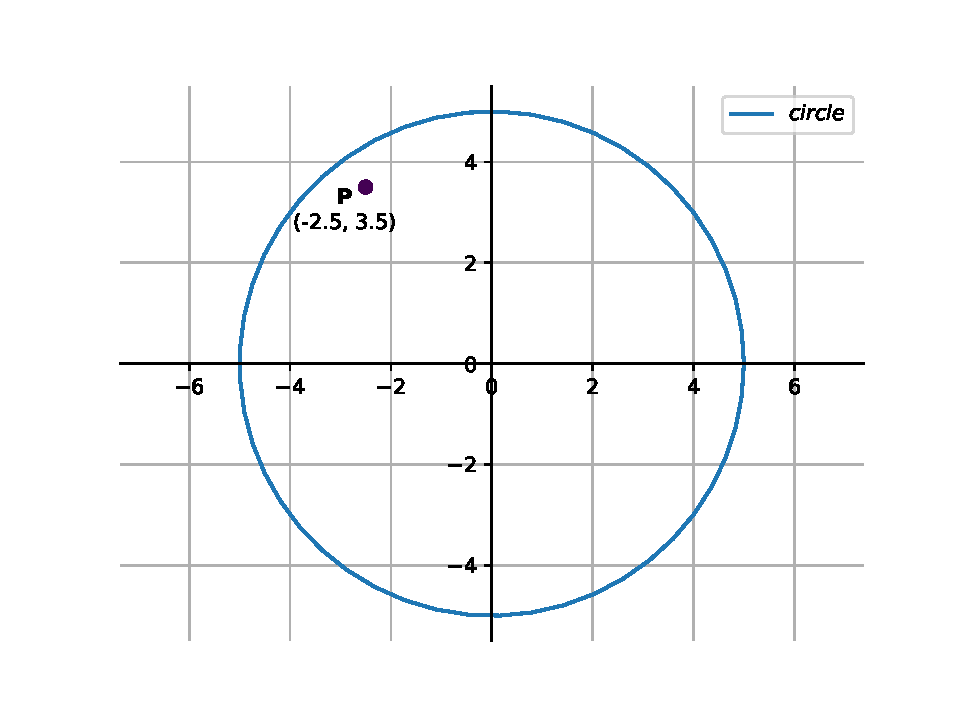
\includegraphics[width=0.75\columnwidth]{chapters/11/11/1/15/figs/fig.pdf}
    \caption{}
    \label{fig:chapters/11/11/1/15/}
\end{figure}
